% shared preamble of the theory figures (white background, purple / black theme, sans-serif)
\documentclass[tikz,border=8pt]{standalone}
\usepackage[T1]{fontenc}
\usepackage[scaled=0.92]{helvet}
\renewcommand{\familydefault}{\sfdefault}
\usepackage{amsmath,amssymb}
\usepackage[helvet]{sfmath}
\usetikzlibrary{arrows.meta,calc,decorations.pathreplacing,positioning,backgrounds}
\definecolor{ink}{HTML}{1A1A1F}
\definecolor{cohesin}{HTML}{6A3DE8}
\definecolor{condensin}{HTML}{1BAF7A}
\definecolor{fwd}{HTML}{D1303F}      % CTCF pointing right
\definecolor{rev}{HTML}{2B62D9}      % CTCF pointing left
\definecolor{panel}{HTML}{F8F6FD}
\definecolor{panelline}{HTML}{E3DDF5}
\tikzset{
  fiber/.style={line width=2.1pt,ink,line cap=round,line join=round},
  halo/.style={line width=6pt,white,line cap=round},
  lab/.style={font=\small,text=ink},
  note/.style={font=\footnotesize,text=ink!60},
  hd/.style={font=\bfseries\small,text=ink,anchor=west},
  leader/.style={line width=0.6pt,ink!45},
}
% soft panel, numbered badge, heading
\newcommand{\panelbg}[4]{\draw[rounded corners=9pt,fill=panel,draw=panelline,line width=0.9pt] (#1,#2) rectangle (#3,#4);}
\newcommand{\badge}[3]{\fill[ink] (#1,#2) circle (0.21);\node[white,font=\bfseries\footnotesize] at (#1,#2) {#3};}
% CTCF: a protein on the fibre carrying an arrow that gives the motif direction (f = right, r = left)
\newcommand{\protf}[2]{\draw[rounded corners=3.5pt,line width=0.6pt,draw=fwd!65!black,fill=fwd] (#1-0.3,#2-0.19) rectangle (#1+0.3,#2+0.19);
  \draw[white,line width=1.5pt,-{Stealth[length=3.4pt,width=4.4pt]}] (#1-0.15,#2)--(#1+0.16,#2);}
\newcommand{\protr}[2]{\draw[rounded corners=3.5pt,line width=0.6pt,draw=rev!65!black,fill=rev] (#1-0.3,#2-0.19) rectangle (#1+0.3,#2+0.19);
  \draw[white,line width=1.5pt,-{Stealth[length=3.4pt,width=4.4pt]}] (#1+0.15,#2)--(#1-0.16,#2);}
\newcommand{\prot}[3]{\csname prot#3\endcsname{#1}{#2}}
% ring seen at an angle, drawn as a tube (dark outline, light core); back half and front half
\newcommand{\ringpart}[5]{\draw[line width=4.6pt,#3!80!black,line cap=round] ([shift={(#1,#2)}]#4:0.55 and 0.21) arc[start angle=#4,end angle=#5,x radius=0.55,y radius=0.21];
  \draw[line width=2.4pt,#3!55!white,line cap=round] ([shift={(#1,#2)}]#4:0.55 and 0.21) arc[start angle=#4,end angle=#5,x radius=0.55,y radius=0.21];}
\newcommand{\ringback}[3]{\ringpart{#1}{#2}{#3}{180}{0}}
\newcommand{\ringfront}[3]{\ringpart{#1}{#2}{#3}{180}{360}}
% smooth loop whose foot (ring) is at (cx,y0): half-width W, height H, ring colour
\newcommand{\lloop}[5]{%
  \ringback{#1}{#2}{#5}%
  \draw[fiber] (#1-0.3,#2) .. controls (#1-0.3,#2+0.25*#4) and (#1-#3,#2+0.2*#4) .. (#1-#3,#2+0.55*#4)
     .. controls (#1-#3,#2+0.95*#4) and (#1-0.5*#3,#2+#4) .. (#1,#2+#4)
     .. controls (#1+0.5*#3,#2+#4) and (#1+#3,#2+0.95*#4) .. (#1+#3,#2+0.55*#4)
     .. controls (#1+#3,#2+0.2*#4) and (#1+0.3,#2+0.25*#4) .. (#1+0.3,#2);%
  \ringfront{#1}{#2}{#5}}
% gently undulating fibre from x0 to the loop foot at cx (height y0), and from x1
\newcommand{\base}[4]{%
  \draw[fiber] plot[smooth] coordinates {(#1,0.05) (#1+0.35*#3-0.35*#1,-0.05) (#3-1.4,0.04)} .. controls (#3-0.6,0.02) and (#3-0.3,0.05) .. (#3-0.3,#4);
  \draw[fiber] plot[smooth] coordinates {(#2,-0.05) (#2-0.35*#2+0.35*#3,0.05) (#3+1.4,-0.04)} .. controls (#3+0.6,-0.02) and (#3+0.3,0.05) .. (#3+0.3,#4);}
% stop sign for a blocked leg and a leg arrow
\newcommand{\stopbar}[3]{\draw[#3,line width=2.4pt,line cap=round] (#1,#2-0.2)--(#1,#2+0.2);}
\newcommand{\legarrow}[3]{\draw[cohesin,line width=1.6pt,-{Stealth[length=5pt,width=6pt]},line cap=round] (#1,#3)--(#2,#3);}

\definecolor{A}{HTML}{D1303F}\definecolor{B}{HTML}{5B4FD6}
\tikzset{ln/.style={line width=0.7pt,ink!45},cur/.style={line width=1.8pt,cohesin},thin/.style={line width=0.9pt},
  mv/.style={line width=1.2pt,ink!70,-{Stealth[length=5pt,width=6pt]}},box/.style={rounded corners=5pt,draw=cohesin!70,fill=white,line width=0.9pt,align=center,font=\small,text=ink,inner sep=4pt}}
\begin{document}
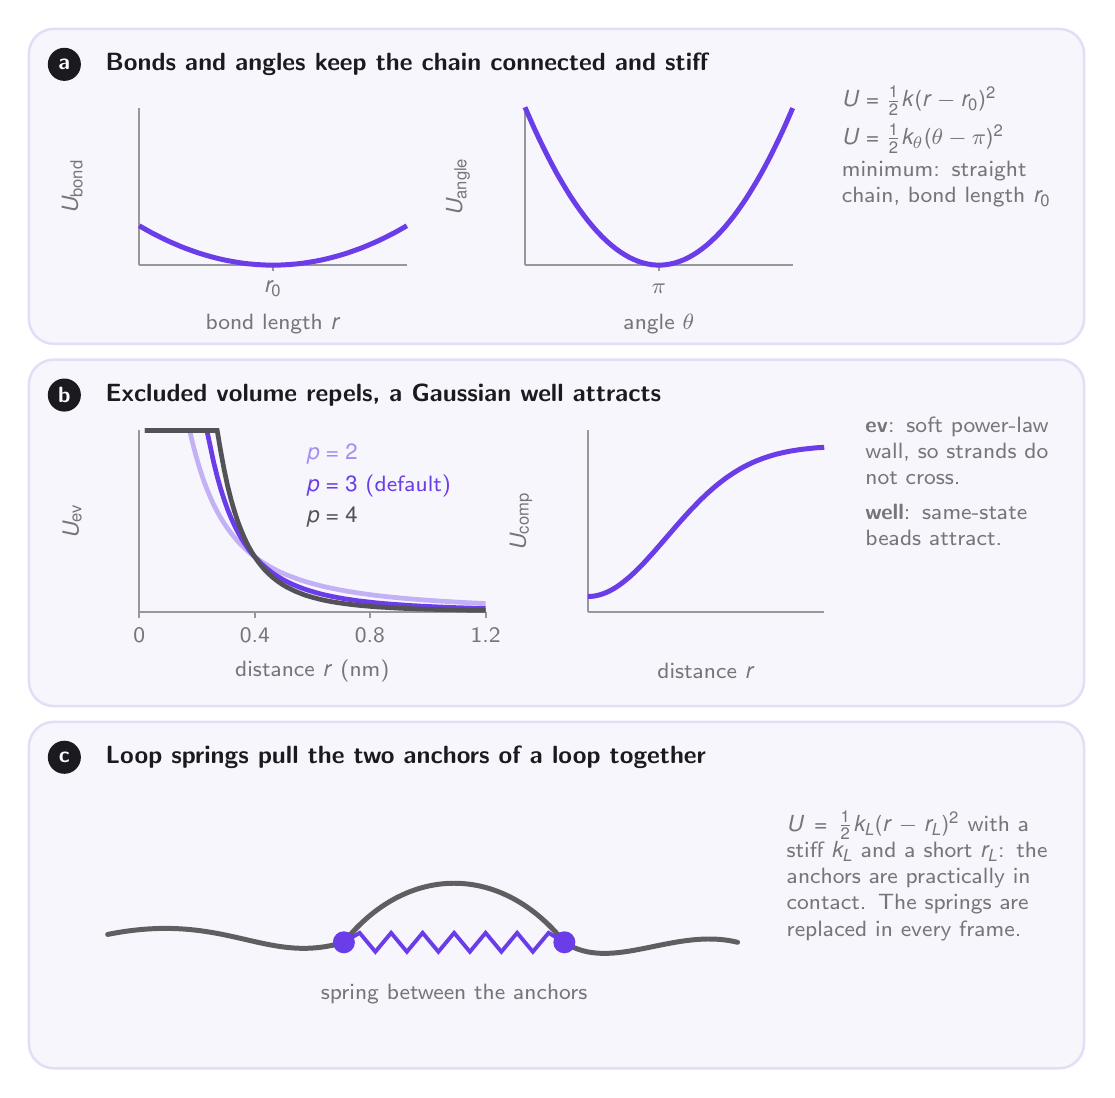
\begin{tikzpicture}
  \panelbg{0}{8.6}{13.4}{12.6}\badge{0.45}{12.15}{a}\node[hd] at (0.85,12.15) {Bonds and angles keep the chain connected and stiff};
  \panelbg{0}{4.0}{13.4}{8.4}\badge{0.45}{7.95}{b}\node[hd] at (0.85,7.95) {Excluded volume repels, a Gaussian well attracts};
  \panelbg{0}{-0.6}{13.4}{3.8}\badge{0.45}{3.3499999999999996}{c}\node[hd] at (0.85,3.3499999999999996) {Loop springs pull the two anchors of a loop together};
  \draw[ln] (1.4,9.6)--(4.8,9.6);\draw[ln] (1.4,9.6)--(1.4,11.6);
  \draw[ln] (3.10,9.6)--(3.10,9.52);\node[note] at (3.10,9.299999999999999) {$r_0$};
  \node[note] at (3.10,8.85) {bond length $r$};
  \node[note,rotate=90] at (0.55,10.60) {$U_{\mathrm{bond}}$};
  \draw[cur] plot coordinates {(1.400,10.100) (1.458,10.067) (1.515,10.035) (1.573,10.003) (1.631,9.974) (1.688,9.945) (1.746,9.917) (1.803,9.891) (1.861,9.866) (1.919,9.841) (1.976,9.818) (2.034,9.797) (2.092,9.776) (2.149,9.756) (2.207,9.738) (2.264,9.721) (2.322,9.705) (2.380,9.690) (2.437,9.676) (2.495,9.663) (2.553,9.652) (2.610,9.642) (2.668,9.632) (2.725,9.624) (2.783,9.617) (2.841,9.612) (2.898,9.607) (2.956,9.604) (3.014,9.601) (3.071,9.600) (3.129,9.600) (3.186,9.601) (3.244,9.604) (3.302,9.607) (3.359,9.612) (3.417,9.617) (3.475,9.624) (3.532,9.632) (3.590,9.642) (3.647,9.652) (3.705,9.663) (3.763,9.676) (3.820,9.690) (3.878,9.705) (3.936,9.721) (3.993,9.738) (4.051,9.756) (4.108,9.776) (4.166,9.797) (4.224,9.818) (4.281,9.841) (4.339,9.866) (4.397,9.891) (4.454,9.917) (4.512,9.945) (4.569,9.974) (4.627,10.003) (4.685,10.035) (4.742,10.067) (4.800,10.100)};
  \draw[ln] (6.3,9.6)--(9.7,9.6);\draw[ln] (6.3,9.6)--(6.3,11.6);
  \draw[ln] (8.00,9.6)--(8.00,9.52);\node[note] at (8.00,9.299999999999999) {$\pi$};
  \node[note] at (8.00,8.85) {angle $\theta$};
  \node[note,rotate=90] at (5.45,10.60) {$U_{\mathrm{angle}}$};
  \draw[cur] plot coordinates {(6.300,11.605) (6.358,11.472) (6.415,11.343) (6.473,11.218) (6.531,11.099) (6.588,10.984) (6.646,10.873) (6.703,10.767) (6.761,10.666) (6.819,10.569) (6.876,10.477) (6.934,10.390) (6.992,10.307) (7.049,10.229) (7.107,10.155) (7.164,10.086) (7.222,10.021) (7.280,9.961) (7.337,9.906) (7.395,9.855) (7.453,9.809) (7.510,9.768) (7.568,9.731) (7.625,9.698) (7.683,9.671) (7.741,9.647) (7.798,9.629) (7.856,9.615) (7.914,9.605) (7.971,9.601) (8.029,9.600) (8.086,9.605) (8.144,9.614) (8.202,9.627) (8.259,9.646) (8.317,9.668) (8.375,9.696) (8.432,9.728) (8.490,9.764) (8.547,9.806) (8.605,9.851) (8.663,9.902) (8.720,9.957) (8.778,10.016) (8.836,10.080) (8.893,10.149) (8.951,10.222) (9.008,10.300) (9.066,10.383) (9.124,10.470) (9.181,10.562) (9.239,10.658) (9.297,10.759) (9.354,10.864) (9.412,10.974) (9.469,11.089) (9.527,11.208) (9.585,11.332) (9.642,11.461) (9.700,11.594)};
  \node[note,text width=3.0cm,anchor=north west] at (10.2,12.0) {$U=\tfrac12k(r-r_0)^2$\\[2pt]$U=\tfrac12k_\theta(\theta-\pi)^2$\\[2pt]minimum: straight chain, bond length $r_0$};
  \draw[ln] (1.4,5.2)--(5.800000000000001,5.2);\draw[ln] (1.4,5.2)--(1.4,7.5);
  \draw[ln] (1.40,5.2)--(1.40,5.12);\node[note] at (1.40,4.9) {0};
  \draw[ln] (2.87,5.2)--(2.87,5.12);\node[note] at (2.87,4.9) {0.4};
  \draw[ln] (4.33,5.2)--(4.33,5.12);\node[note] at (4.33,4.9) {0.8};
  \draw[ln] (5.80,5.2)--(5.80,5.12);\node[note] at (5.80,4.9) {1.2};
  \node[note] at (3.60,4.45) {distance $r$ (nm)};
  \node[note,rotate=90] at (0.55,6.35) {$U_{\mathrm{ev}}$};
  \draw[line width=1.7pt,cohesin!40] plot coordinates {(1.473,7.500) (1.517,7.500) (1.561,7.500) (1.604,7.500) (1.648,7.500) (1.692,7.500) (1.736,7.500) (1.779,7.500) (1.823,7.500) (1.867,7.500) (1.910,7.500) (1.954,7.500) (1.998,7.500) (2.041,7.500) (2.085,7.317) (2.129,7.152) (2.173,7.005) (2.216,6.874) (2.260,6.757) (2.304,6.652) (2.347,6.557) (2.391,6.471) (2.435,6.393) (2.479,6.322) (2.522,6.257) (2.566,6.197) (2.610,6.143) (2.653,6.093) (2.697,6.046) (2.741,6.004) (2.784,5.964) (2.828,5.927) (2.872,5.893) (2.916,5.861) (2.959,5.832) (3.003,5.804) (3.047,5.778) (3.090,5.754) (3.134,5.731) (3.178,5.709) (3.221,5.689) (3.265,5.670) (3.309,5.652) (3.353,5.636) (3.396,5.620) (3.440,5.604) (3.484,5.590) (3.527,5.577) (3.571,5.564) (3.615,5.552) (3.659,5.540) (3.702,5.529) (3.746,5.518) (3.790,5.508) (3.833,5.499) (3.877,5.490) (3.921,5.481) (3.964,5.473) (4.008,5.465) (4.052,5.457) (4.096,5.450) (4.139,5.443) (4.183,5.436) (4.227,5.430) (4.270,5.424) (4.314,5.418) (4.358,5.412) (4.401,5.406) (4.445,5.401) (4.489,5.396) (4.533,5.391) (4.576,5.387) (4.620,5.382) (4.664,5.378) (4.707,5.374) (4.751,5.369) (4.795,5.366) (4.839,5.362) (4.882,5.358) (4.926,5.355) (4.970,5.351) (5.013,5.348) (5.057,5.345) (5.101,5.342) (5.144,5.339) (5.188,5.336) (5.232,5.333) (5.276,5.330) (5.319,5.328) (5.363,5.325) (5.407,5.322) (5.450,5.320) (5.494,5.318) (5.538,5.315) (5.581,5.313) (5.625,5.311) (5.669,5.309) (5.713,5.307) (5.756,5.305) (5.800,5.303)};
  \draw[line width=1.7pt,cohesin] plot coordinates {(1.473,7.500) (1.517,7.500) (1.561,7.500) (1.604,7.500) (1.648,7.500) (1.692,7.500) (1.736,7.500) (1.779,7.500) (1.823,7.500) (1.867,7.500) (1.910,7.500) (1.954,7.500) (1.998,7.500) (2.041,7.500) (2.085,7.500) (2.129,7.500) (2.173,7.500) (2.216,7.500) (2.260,7.500) (2.304,7.295) (2.347,7.093) (2.391,6.916) (2.435,6.760) (2.479,6.623) (2.522,6.501) (2.566,6.393) (2.610,6.297) (2.653,6.210) (2.697,6.133) (2.741,6.063) (2.784,6.000) (2.828,5.943) (2.872,5.891) (2.916,5.844) (2.959,5.801) (3.003,5.762) (3.047,5.726) (3.090,5.693) (3.134,5.663) (3.178,5.636) (3.221,5.610) (3.265,5.586) (3.309,5.564) (3.353,5.544) (3.396,5.526) (3.440,5.508) (3.484,5.492) (3.527,5.477) (3.571,5.463) (3.615,5.450) (3.659,5.437) (3.702,5.426) (3.746,5.415) (3.790,5.405) (3.833,5.396) (3.877,5.387) (3.921,5.378) (3.964,5.371) (4.008,5.363) (4.052,5.356) (4.096,5.350) (4.139,5.343) (4.183,5.337) (4.227,5.332) (4.270,5.327) (4.314,5.322) (4.358,5.317) (4.401,5.312) (4.445,5.308) (4.489,5.304) (4.533,5.300) (4.576,5.297) (4.620,5.293) (4.664,5.290) (4.707,5.287) (4.751,5.284) (4.795,5.281) (4.839,5.278) (4.882,5.275) (4.926,5.273) (4.970,5.270) (5.013,5.268) (5.057,5.266) (5.101,5.264) (5.144,5.262) (5.188,5.260) (5.232,5.258) (5.276,5.256) (5.319,5.255) (5.363,5.253) (5.407,5.251) (5.450,5.250) (5.494,5.248) (5.538,5.247) (5.581,5.246) (5.625,5.244) (5.669,5.243) (5.713,5.242) (5.756,5.241) (5.800,5.240)};
  \draw[line width=1.7pt,ink!75] plot coordinates {(1.473,7.500) (1.517,7.500) (1.561,7.500) (1.604,7.500) (1.648,7.500) (1.692,7.500) (1.736,7.500) (1.779,7.500) (1.823,7.500) (1.867,7.500) (1.910,7.500) (1.954,7.500) (1.998,7.500) (2.041,7.500) (2.085,7.500) (2.129,7.500) (2.173,7.500) (2.216,7.500) (2.260,7.500) (2.304,7.500) (2.347,7.500) (2.391,7.500) (2.435,7.241) (2.479,7.005) (2.522,6.802) (2.566,6.627) (2.610,6.475) (2.653,6.343) (2.697,6.228) (2.741,6.126) (2.784,6.037) (2.828,5.959) (2.872,5.889) (2.916,5.827) (2.959,5.772) (3.003,5.723) (3.047,5.679) (3.090,5.640) (3.134,5.604) (3.178,5.572) (3.221,5.543) (3.265,5.517) (3.309,5.494) (3.353,5.472) (3.396,5.453) (3.440,5.435) (3.484,5.418) (3.527,5.403) (3.571,5.390) (3.615,5.377) (3.659,5.366) (3.702,5.355) (3.746,5.345) (3.790,5.336) (3.833,5.328) (3.877,5.320) (3.921,5.313) (3.964,5.307) (4.008,5.301) (4.052,5.295) (4.096,5.290) (4.139,5.285) (4.183,5.280) (4.227,5.276) (4.270,5.272) (4.314,5.268) (4.358,5.264) (4.401,5.261) (4.445,5.258) (4.489,5.255) (4.533,5.253) (4.576,5.250) (4.620,5.248) (4.664,5.245) (4.707,5.243) (4.751,5.241) (4.795,5.239) (4.839,5.238) (4.882,5.236) (4.926,5.234) (4.970,5.233) (5.013,5.231) (5.057,5.230) (5.101,5.229) (5.144,5.228) (5.188,5.226) (5.232,5.225) (5.276,5.224) (5.319,5.223) (5.363,5.222) (5.407,5.222) (5.450,5.221) (5.494,5.220) (5.538,5.219) (5.581,5.218) (5.625,5.218) (5.669,5.217) (5.713,5.216) (5.756,5.216) (5.800,5.215)};
  \node[note,anchor=west,text=cohesin!60] at (3.4,7.2) {$p=2$};\node[note,anchor=west,text=cohesin] at (3.4,6.8) {$p=3$ (default)};\node[note,anchor=west,text=ink!75] at (3.4,6.4) {$p=4$};
  \draw[ln] (7.1,5.2)--(10.1,5.2);\draw[ln] (7.1,5.2)--(7.1,7.5);
  \node[note] at (8.60,4.45) {distance $r$};
  \node[note,rotate=90] at (6.25,6.35) {$U_{\mathrm{comp}}$};
  \draw[cur] plot coordinates {(7.100,5.392) (7.138,5.393) (7.176,5.397) (7.214,5.404) (7.252,5.414) (7.290,5.426) (7.328,5.441) (7.366,5.458) (7.404,5.478) (7.442,5.500) (7.480,5.525) (7.518,5.552) (7.556,5.581) (7.594,5.612) (7.632,5.644) (7.670,5.679) (7.708,5.715) (7.746,5.752) (7.784,5.791) (7.822,5.831) (7.859,5.872) (7.897,5.914) (7.935,5.956) (7.973,5.999) (8.011,6.043) (8.049,6.087) (8.087,6.131) (8.125,6.175) (8.163,6.219) (8.201,6.263) (8.239,6.307) (8.277,6.350) (8.315,6.392) (8.353,6.434) (8.391,6.476) (8.429,6.516) (8.467,6.555) (8.505,6.594) (8.543,6.632) (8.581,6.668) (8.619,6.704) (8.657,6.738) (8.695,6.771) (8.733,6.803) (8.771,6.834) (8.809,6.863) (8.847,6.892) (8.885,6.919) (8.923,6.944) (8.961,6.969) (8.999,6.992) (9.037,7.015) (9.075,7.036) (9.113,7.055) (9.151,7.074) (9.189,7.092) (9.227,7.109) (9.265,7.124) (9.303,7.139) (9.341,7.153) (9.378,7.165) (9.416,7.177) (9.454,7.188) (9.492,7.199) (9.530,7.208) (9.568,7.217) (9.606,7.225) (9.644,7.233) (9.682,7.240) (9.720,7.246) (9.758,7.252) (9.796,7.258) (9.834,7.263) (9.872,7.267) (9.910,7.271) (9.948,7.275) (9.986,7.279) (10.024,7.282) (10.062,7.284) (10.100,7.287)};
  \node[note,text width=2.5cm,anchor=north west] at (10.5,7.8) {\textbf{ev}: soft power-law wall, so strands do not cross.\\[3pt]\textbf{well}: same-state beads attract.};
  \begin{scope}[yshift=0.9cm]
  \draw[fiber,ink!70,line width=1.8pt] (1.0,0.2) .. controls (2.5,0.5) and (3.0,-0.2) .. (4.0,0.1);
  \draw[fiber,ink!70,line width=1.8pt] (4.0,0.1) .. controls (4.8,1.1) and (6.0,1.1) .. (6.8,0.1) .. controls (7.4,-0.3) and (8.2,0.3) .. (9.0,0.1);
  \fill[cohesin] (4.0,0.1) circle (0.14);\fill[cohesin] (6.8,0.1) circle (0.14);
  \draw[cohesin,line width=1.4pt] (4.00,0.10) -- (4.20,0.22) -- (4.40,-0.02) -- (4.60,0.22) -- (4.80,-0.02) -- (5.00,0.22) -- (5.20,-0.02) -- (5.40,0.22) -- (5.60,-0.02) -- (5.80,0.22) -- (6.00,-0.02) -- (6.20,0.22) -- (6.40,-0.02) -- (6.60,0.22) -- (6.80,0.10);
  \node[note] at (5.4,-0.55) {spring between the anchors};
  \node[note,text width=3.4cm,anchor=north west] at (9.5,1.9) {$U=\tfrac12k_L(r-r_L)^2$ with a stiff $k_L$ and a short $r_L$: the anchors are practically in contact. The springs are replaced in every frame.};
  \end{scope}
\end{tikzpicture}
\end{document}
